\subsection{Ideation, Formulation and Analysis}

The mixer is a fundamental building block in our quadrature down converter, responsible for frequency translation by multiplying the input signal with the local oscillator (LO) signal. In this project, we implement a simple NMOS-based switching mixer, as shown in Fig.~\ref{fig:nmos_mixer}.

\begin{figure}[H]
    \centering
    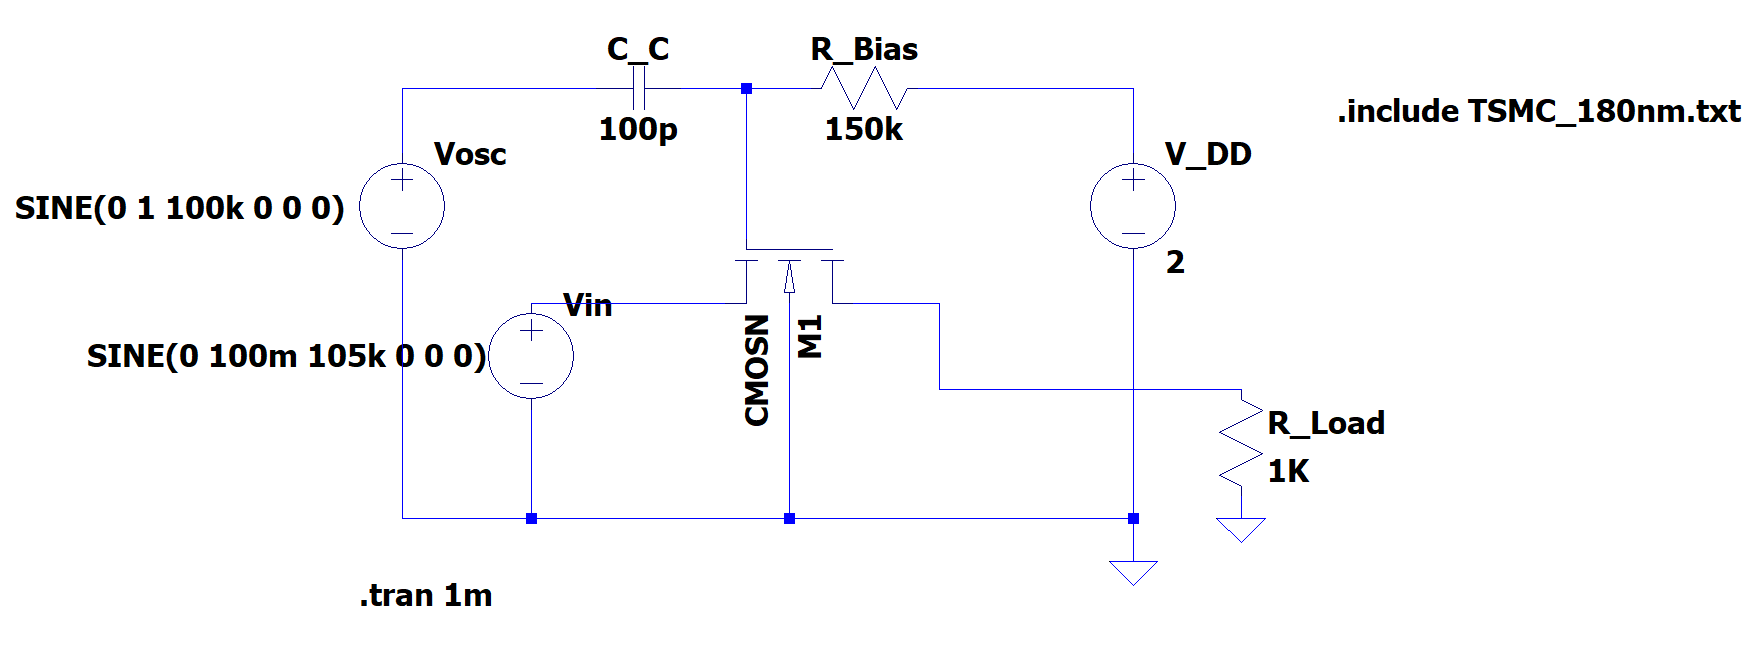
\includegraphics[width=\linewidth]{fig/mixer.png}
    \caption{NMOS Mixer Schematic (LTspice)}
    \label{fig:nmos_mixer}
\end{figure}

\subsubsection{Circuit Configuration}
The mixer consists of:
\begin{itemize}
    \item \textbf{NMOS transistor (M1)}: TSMC 180nm model, acts as the mixing element
    \item \textbf{Coupling capacitor ($C_C = 100$ pF)}: Blocks DC while passing AC oscillator signal
    \item \textbf{Bias resistor ($R_{Bias} = 150$ k$\Omega$)}: Provides DC path for proper gate biasing
    \item \textbf{Load resistor ($R_L = 1$ k$\Omega$)}: Converts drain current to output voltage
    \item \textbf{Input signal}: $V_{in} = 100$ mV amplitude at $(100 + \Delta f)$ kHz
    \item \textbf{Oscillator signal}: $V_{OSC} = 1$ V amplitude at 100 kHz
    \item \textbf{Supply voltage}: $V_{DD} = 2$ V
\end{itemize}
\subsubsection{Component Value Selection}
The component values were carefully chosen to ensure optimal mixer performance:

\begin{itemize}
    \item \textbf{Coupling Capacitor ($C_C = 100$ pF)}
    \begin{itemize}
        \item \textit{Purpose}: Blocks DC while passing AC oscillator signal to gate
        \item \textit{Selection rationale}: Provides low impedance ($\approx 15.9$ k$\Omega$) at 100 kHz
        \item \textit{Desired range}: 10 pF - 1 nF
        \begin{itemize}
            \item Too small ($<$10 pF): High impedance limits signal coupling
            \item Too large ($>$1 nF): Unnecessary physical size, longer discharge time
        \end{itemize}
    \end{itemize}
    
    \item \textbf{Bias Resistor ($R_{Bias} = 150$ k$\Omega$)}
    \begin{itemize}
        \item \textit{Purpose}: Provides DC path to ground for gate biasing
        \item \textit{Selection rationale}: High enough to minimize loading effects on oscillator
        \item \textit{Desired range}: 10 k$\Omega$ - 1 M$\Omega$
        \begin{itemize}
            \item Too small ($<$10 k$\Omega$): Loads oscillator signal, wastes power
            \item Too large ($>$1 M$\Omega$): May cause biasing instability, noise susceptibility
        \end{itemize}
    \end{itemize}
    
    \item \textbf{Load Resistor ($R_L = 1$ k$\Omega$)}
    \begin{itemize}
        \item \textit{Purpose}: Converts drain current variations to voltage
        \item \textit{Selection rationale}: Project requirement, balances output signal level with power consumption
        \item \textit{Desired range}: 100 $\Omega$ - 10 k$\Omega$
        \begin{itemize}
            \item Too small ($<$100 $\Omega$): Excessive current, low output voltage swing
            \item Too large ($>$10 k$\Omega$): Reduced bandwidth due to parasitic capacitances
        \end{itemize}
    \end{itemize}
    
    \item \textbf{Supply Voltage ($V_{DD} = 2$ V)}
    \begin{itemize}
        \item \textit{Purpose}: Powers the circuit, provides headroom for transistor operation
        \item \textit{Selection rationale}: Sufficient for 180 nm CMOS technology
        \item \textit{Desired range}: 1.8 V - 3.3 V
        \begin{itemize}
            \item Too low ($<$1.8 V): Insufficient headroom for proper operation
            \item Too high ($>$3.3 V): Excessive power consumption, potential reliability issues
        \end{itemize}
    \end{itemize}
    
    \item \textbf{Signal Parameters}
    \begin{itemize}
        \item \textit{Input signal} (100 mV): Appropriate level for linear operation
        \begin{itemize}
            \item Range: 10 mV - 500 mV
        \end{itemize}
        \item \textit{Oscillator signal} (1 V): Sufficient amplitude to ensure complete switching
        \begin{itemize}
            \item Range: 0.5 V - 2 V
        \end{itemize}
    \end{itemize}
\end{itemize}

\textbf{Mixer Principle:}  
The NMOS transistor operates as a time-varying resistor, controlled by the LO at its gate. When $V_{GS} > V_{th}$ (positive LO half-cycle), the device enters the triode region, allowing the input signal to pass to the drain. When $V_{GS} < V_{th}$ (negative LO half-cycle), the device is in cutoff and blocks the signal, except for small contributions via parasitic capacitance.

Mixing is mathematically described as:
$$
V_{IF} = V_{in} \times V_{OSC} 
$$
$$V_{IF}= \frac{A_1 A_2}{2} \left[ \cos((\omega_{in} - \omega_{osc})t) + \cos((\omega_{in} + \omega_{osc})t) \right]$$
 
where $A_1$ and $A_2$ are the amplitudes of the input and LO signals.

The mixer in our quadrature down converter performs frequency down-conversion, taking the $(100 + \Delta f)$ kHz input signal and translating it to a $\Delta f$ kHz intermediate frequency by mixing with the 100 kHz local oscillator. This frequency difference is essential for further signal processing in wireless communication systems where high-frequency signals need to be converted to lower frequencies for efficient processing.

\subsection{Simulation and Results}

To verify the performance of our NMOS mixer design, we conducted extensive LTspice simulations using the TSMC 180nm transistor model. The circuit was implemented as shown in Fig.~\ref{fig:nmos_mixer} with the component values specified in the previous section.

\begin{figure}[H]
    \centering
    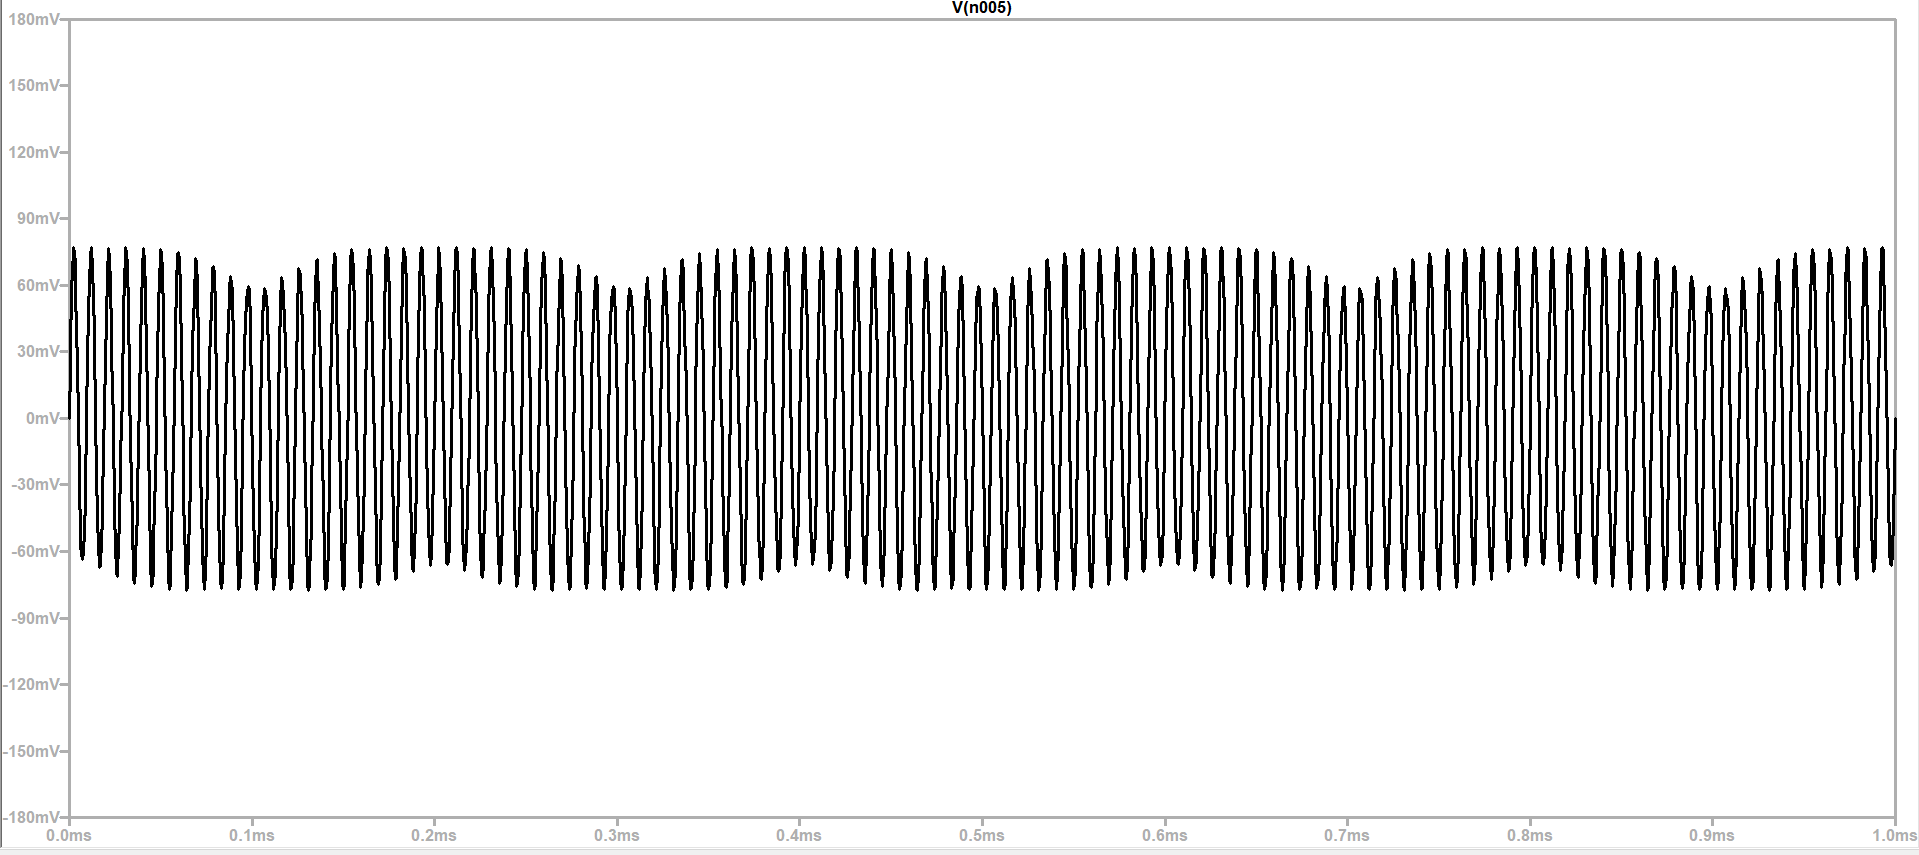
\includegraphics[width=\linewidth]{fig/105.png}
    \caption{Mixer Output Waveform ($V_{IF}$ at drain) for $f_{in} = 105$ kHz ($\Delta f = 5$ kHz)}
    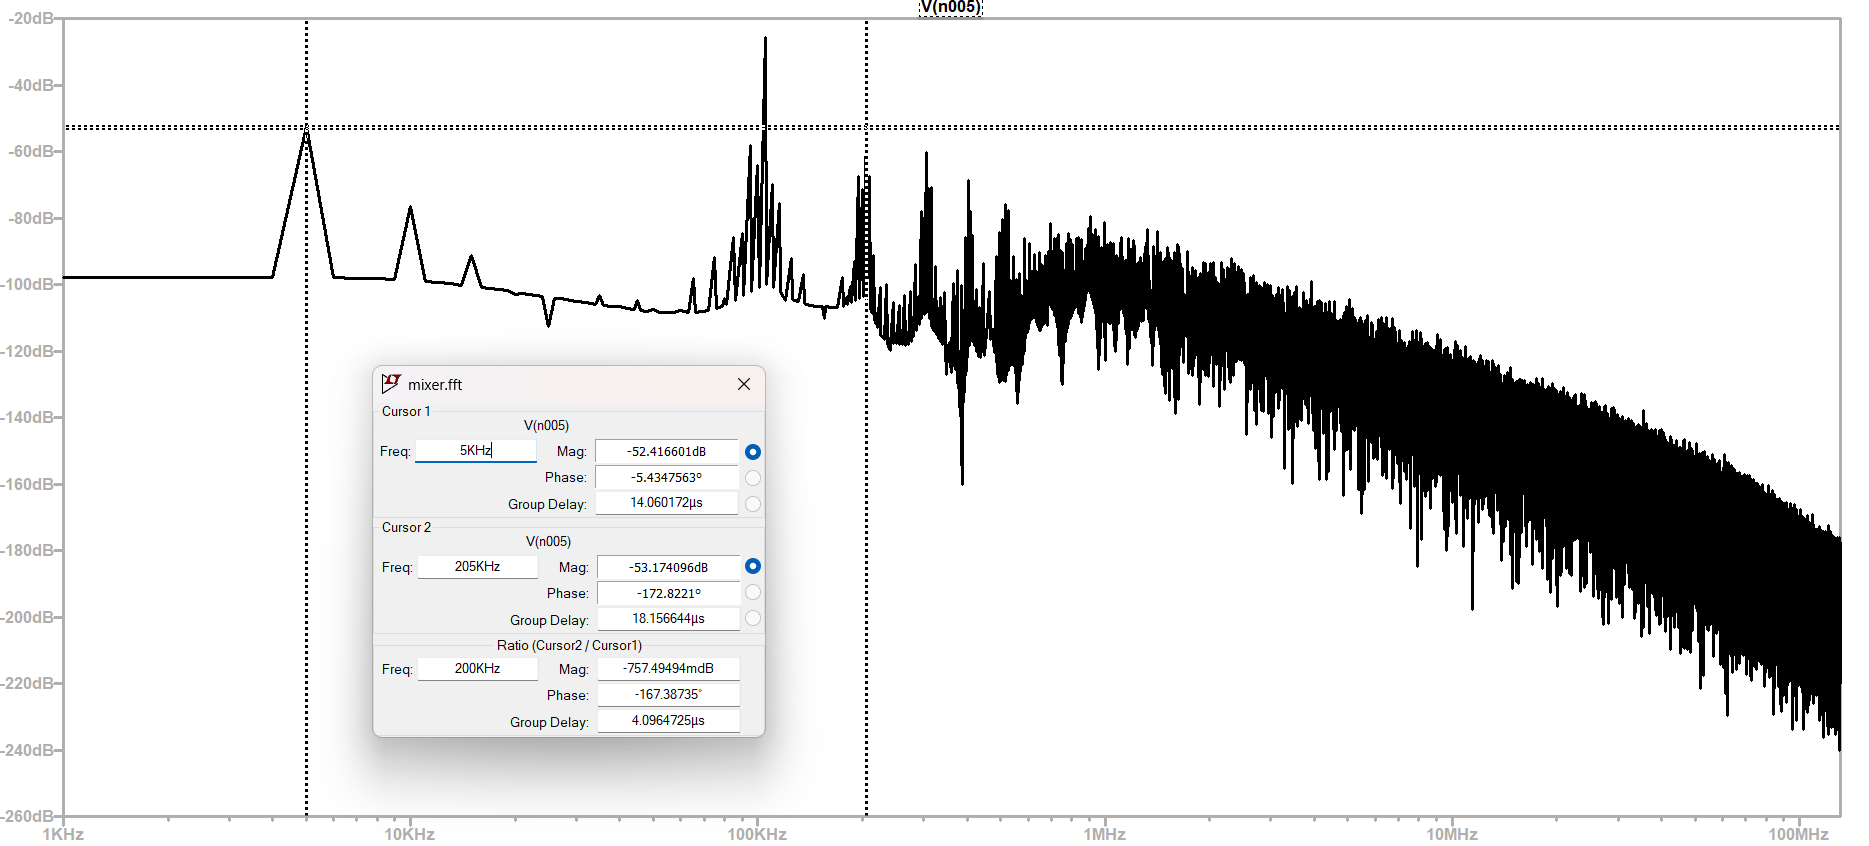
\includegraphics[width=1\linewidth]{fig/105fft.png}
     \caption{105kHz FFT}
    \label{fig:mixer_output}
\end{figure}

As seen in Fig.~\ref{fig:mixer_output}, the output waveform exhibits a clear beat pattern with an envelope frequency of $\Delta f = 5$ kHz, which corresponds to the difference between the input frequency (105 kHz) and the LO frequency (100 kHz). The output signal swings between approximately $-80$ mV and $+80$ mV, indicating a conversion gain of:

$$
G_c = \frac{V_{IF}}{V_{in}} \approx \frac{80\,\text{mV}}{100\,\text{mV}} = 0.8 \approx -1.94\,\text{dB}
$$

This conversion gain is typical for passive MOSFET mixers and demonstrates efficient frequency translation.

To thoroughly analyze the mixer's performance across various input frequencies, we conducted simulations with $f_{in} = \{95, 98, 99, 101, 102, 105\}$ kHz (corresponding to $\Delta f = \{5, 2, 1, 1, 2, 5\}$ kHz) while maintaining $f_{osc} = 100$ kHz. The results demonstrate the following behavior:

\begin{figure}[H]
    \centering
    % Place image of multiple frequency responses here
        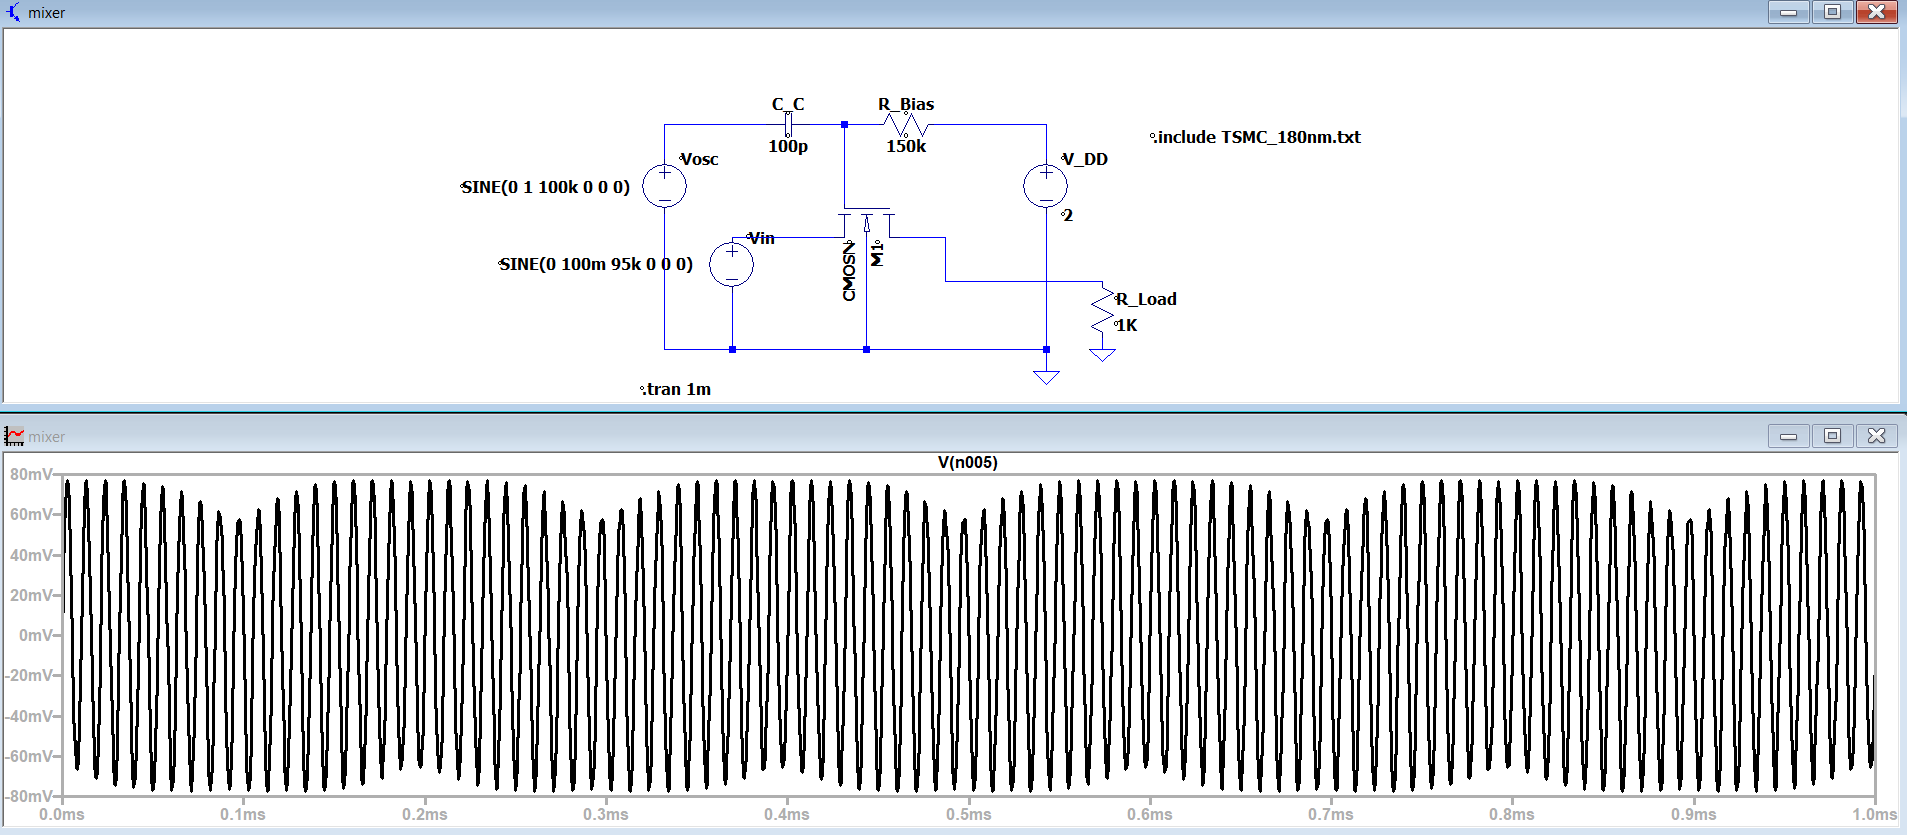
\includegraphics[width=1\linewidth]{fig/95.png}
        \caption{95kHz Output Signal}
         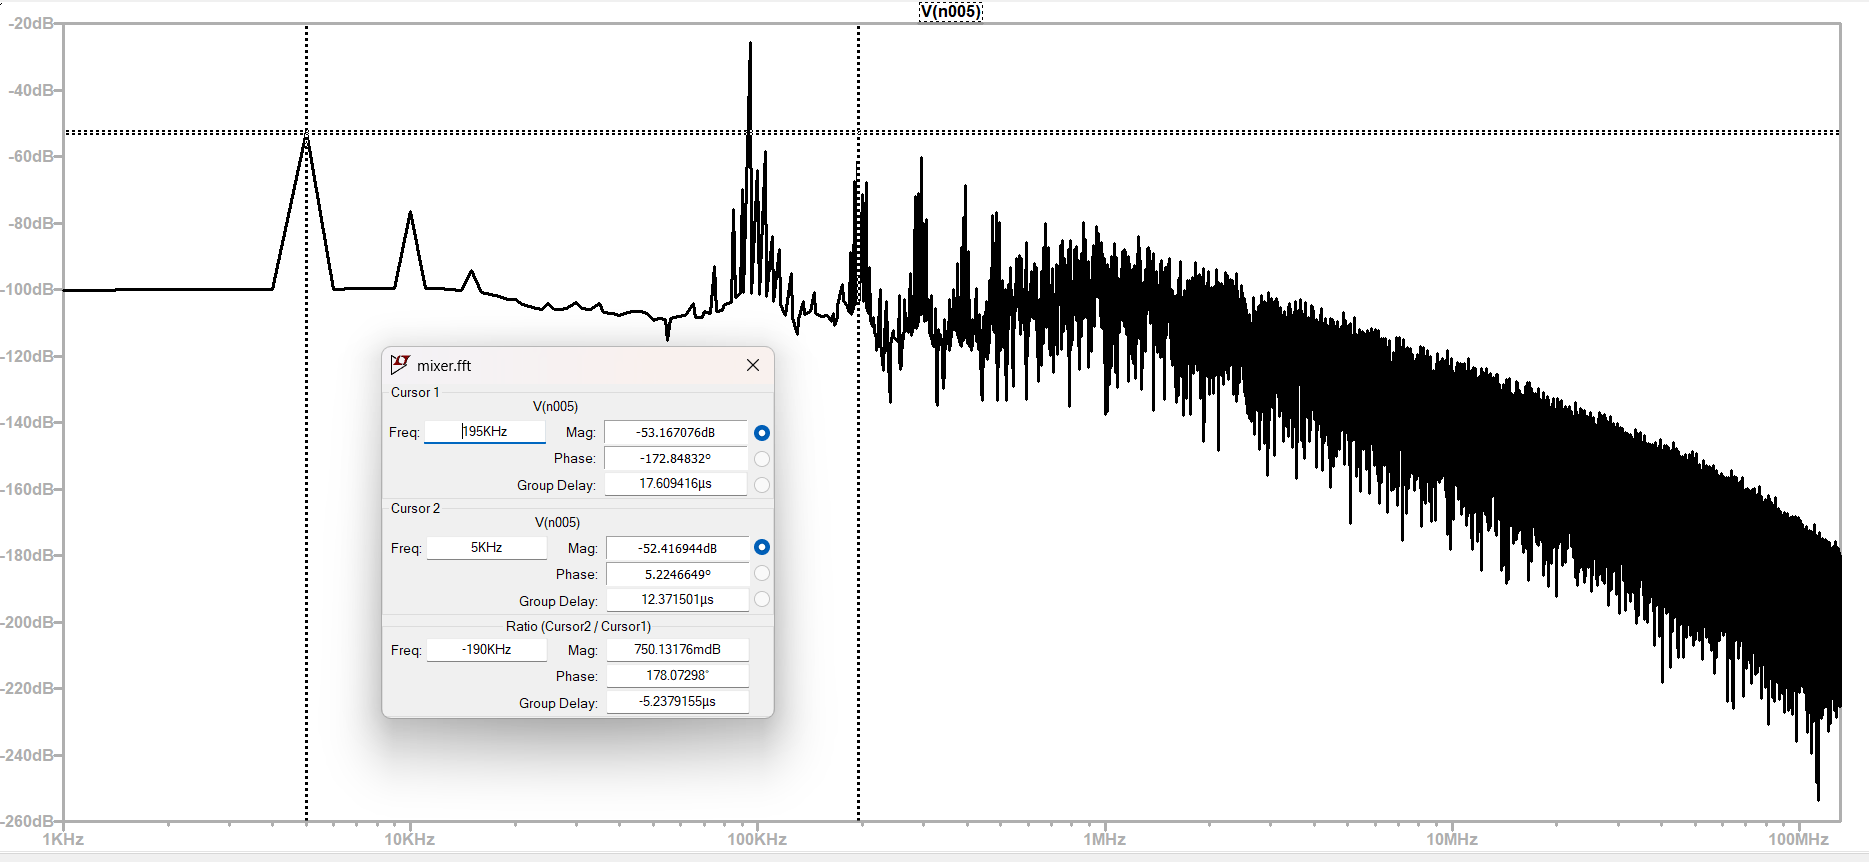
\includegraphics[width=1\linewidth]{fig/95fft.png}
        \caption{95kHz FFT}

\end{figure}
\begin{figure}
    \centering
    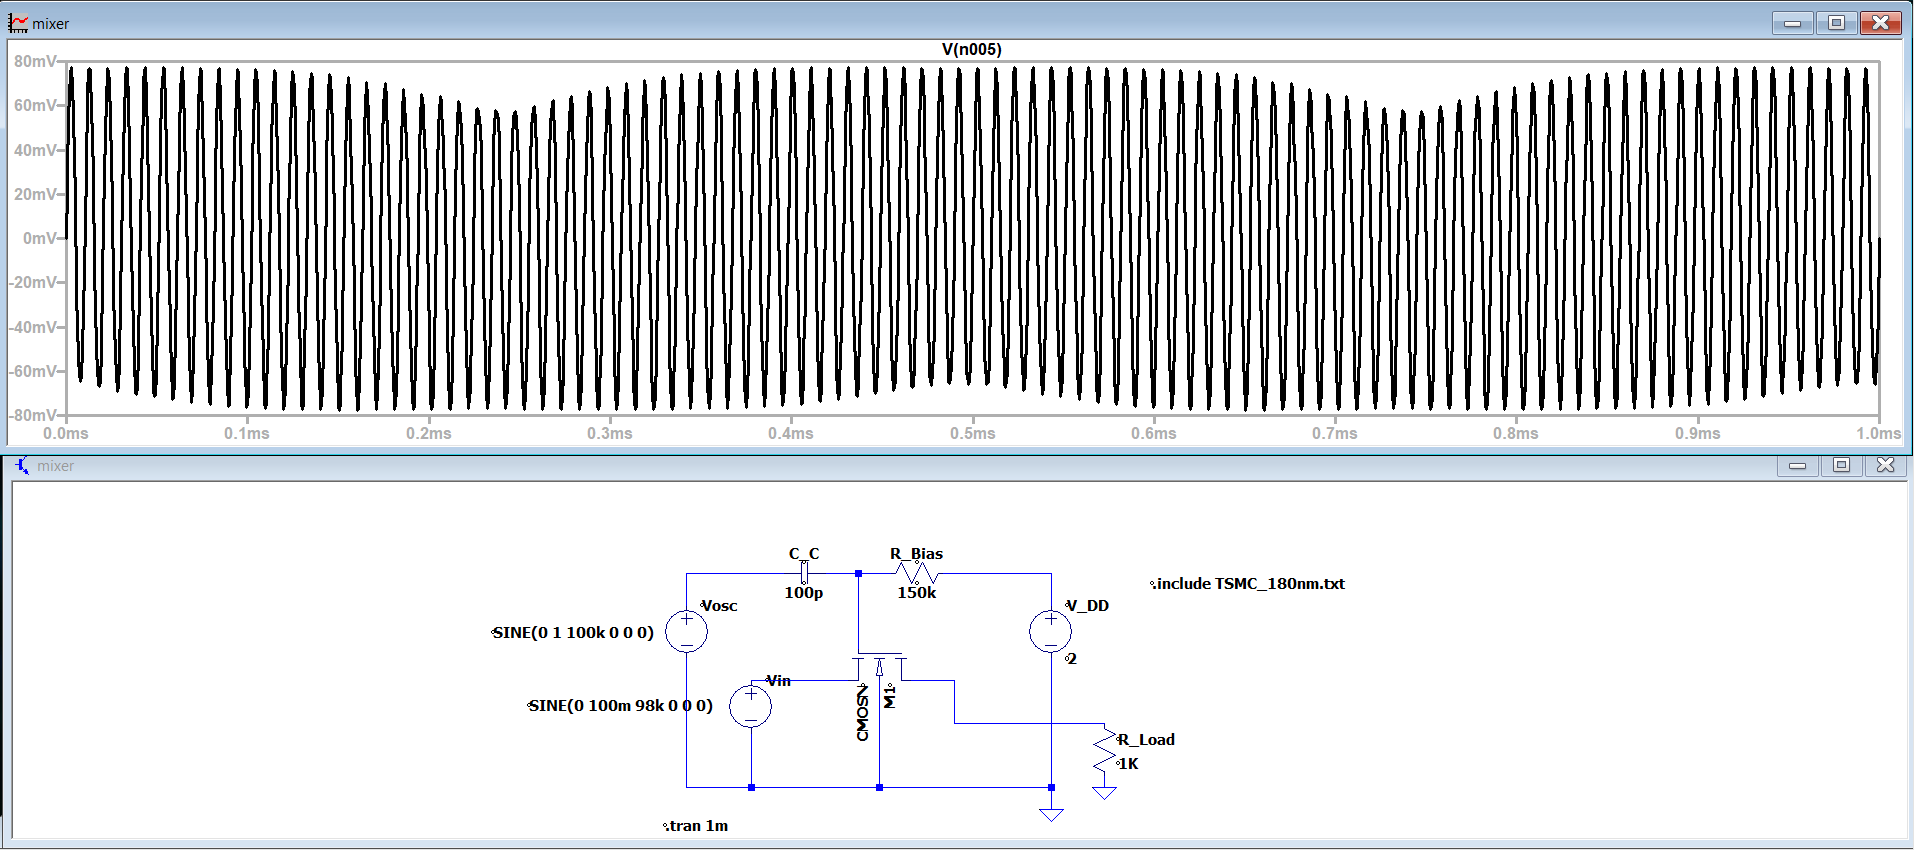
\includegraphics[width=1\linewidth]{fig/98.png}
    \caption{98kHz Output Signal}
    
    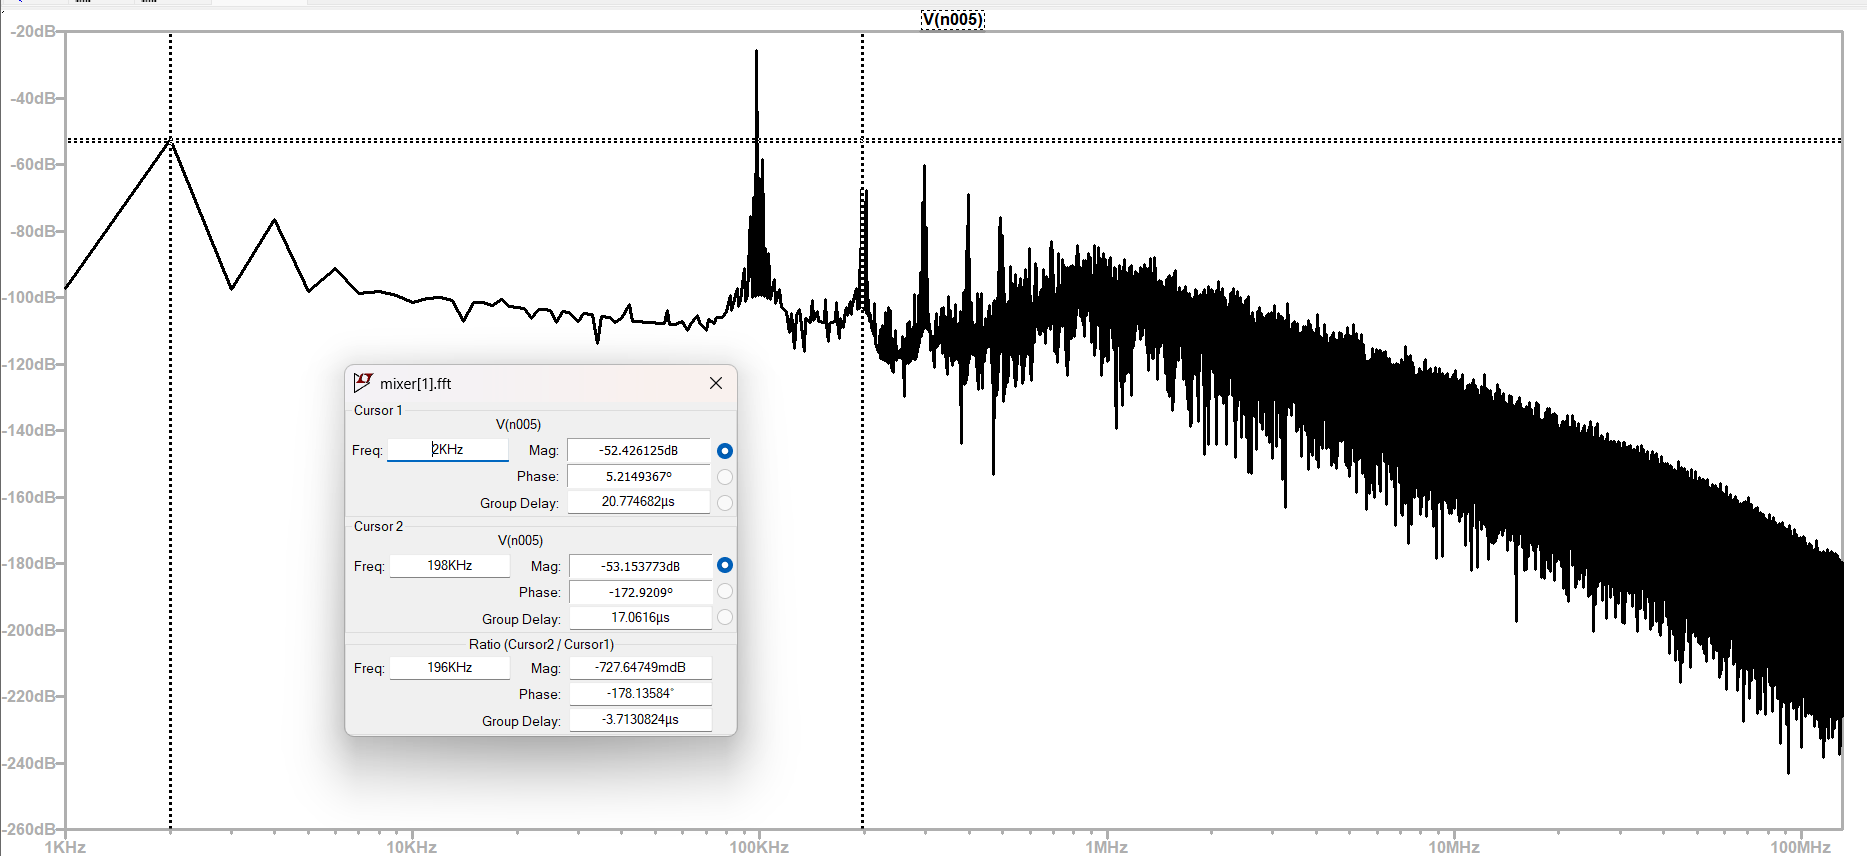
\includegraphics[width=1\linewidth]{98fft.png}
    \caption{98kHz FFT}
\end{figure}
\begin{figure}
    \centering
    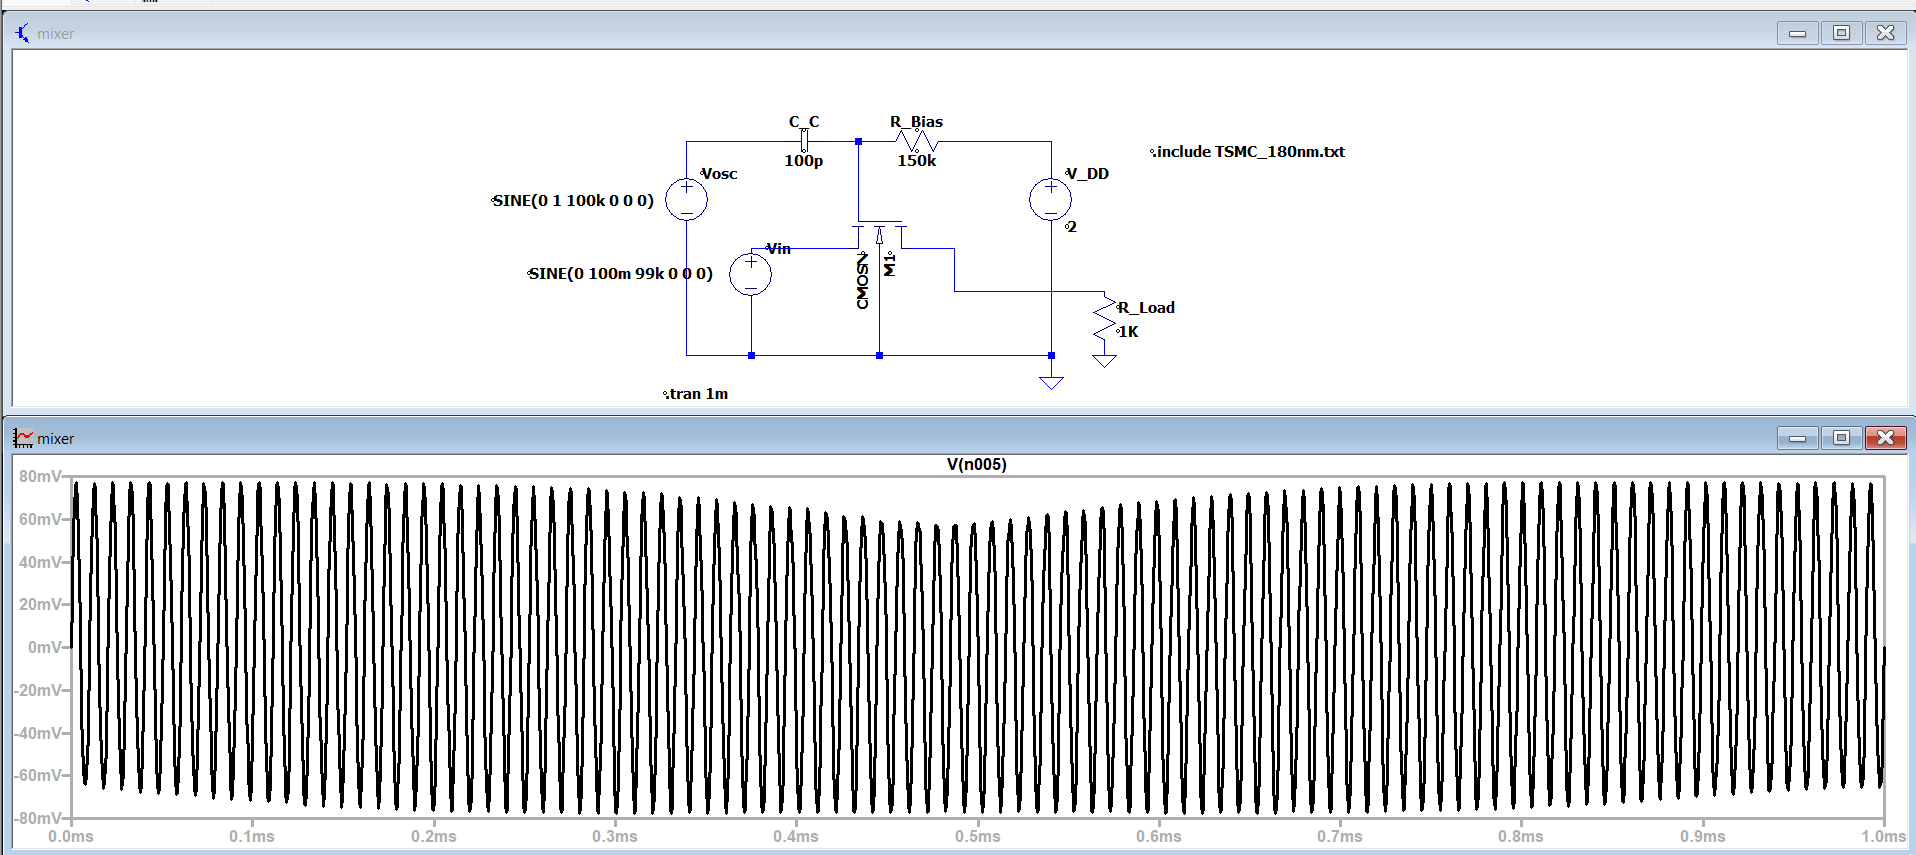
\includegraphics[width=1\linewidth]{fig/99.png}
    \caption{99kHz Output Signal}
    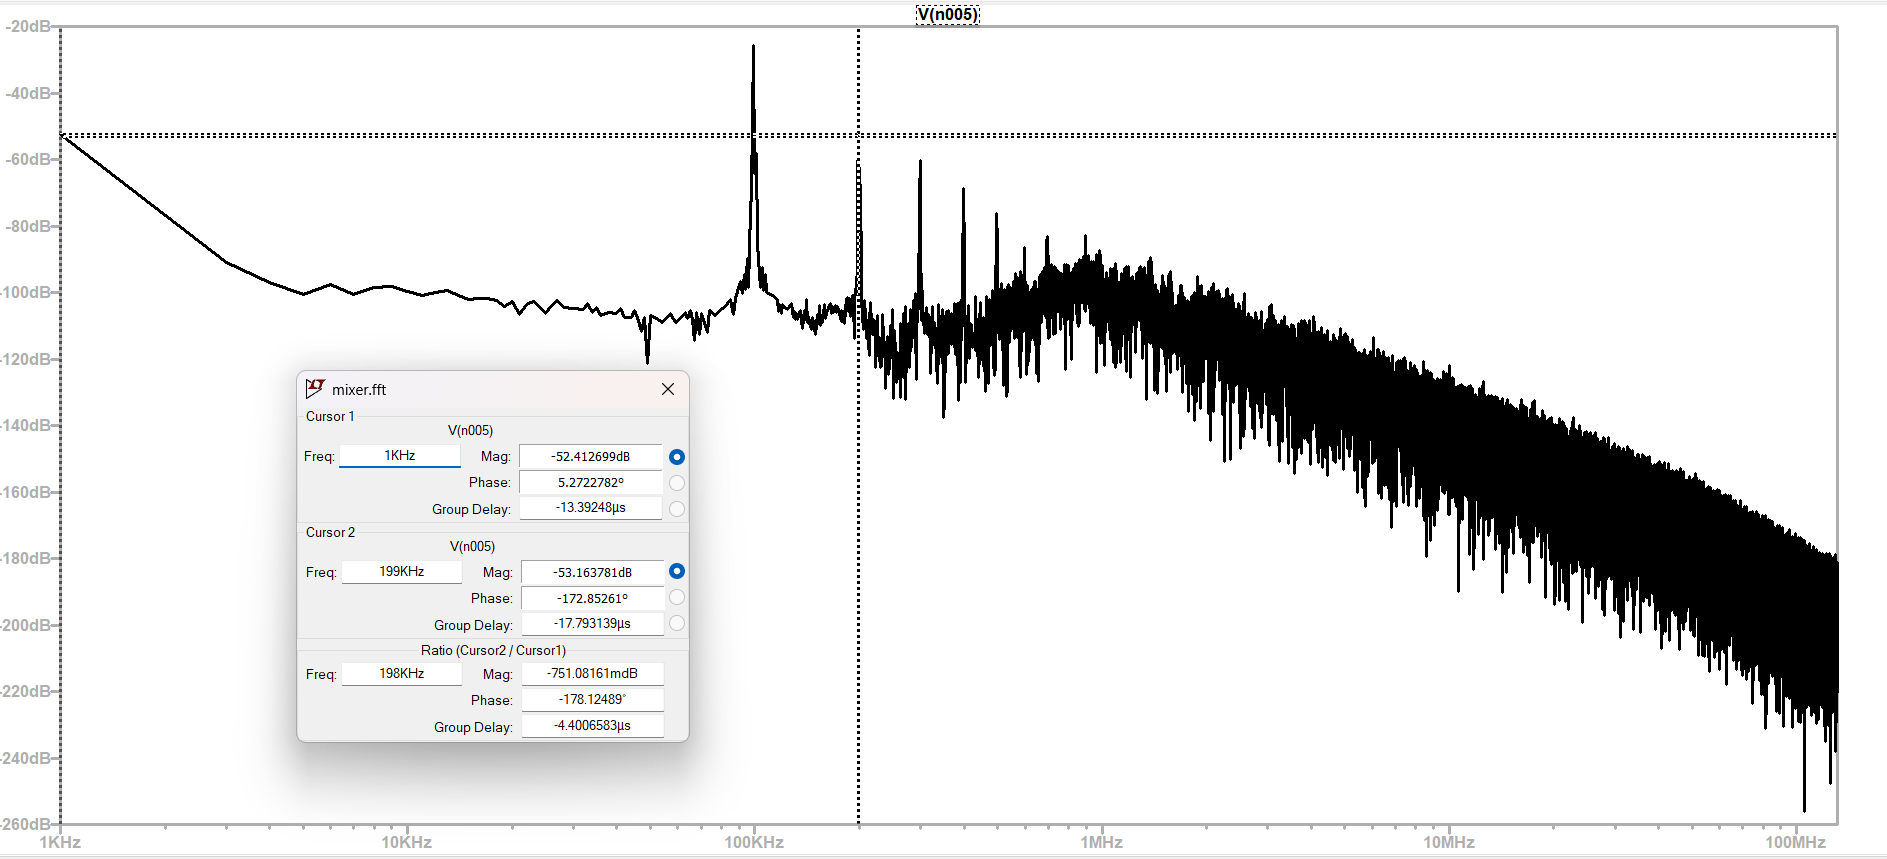
\includegraphics[width=1\linewidth]{fig/99fft.png}
    \caption{99kHz FFT}
\end{figure}
\begin{figure}
    \centering
    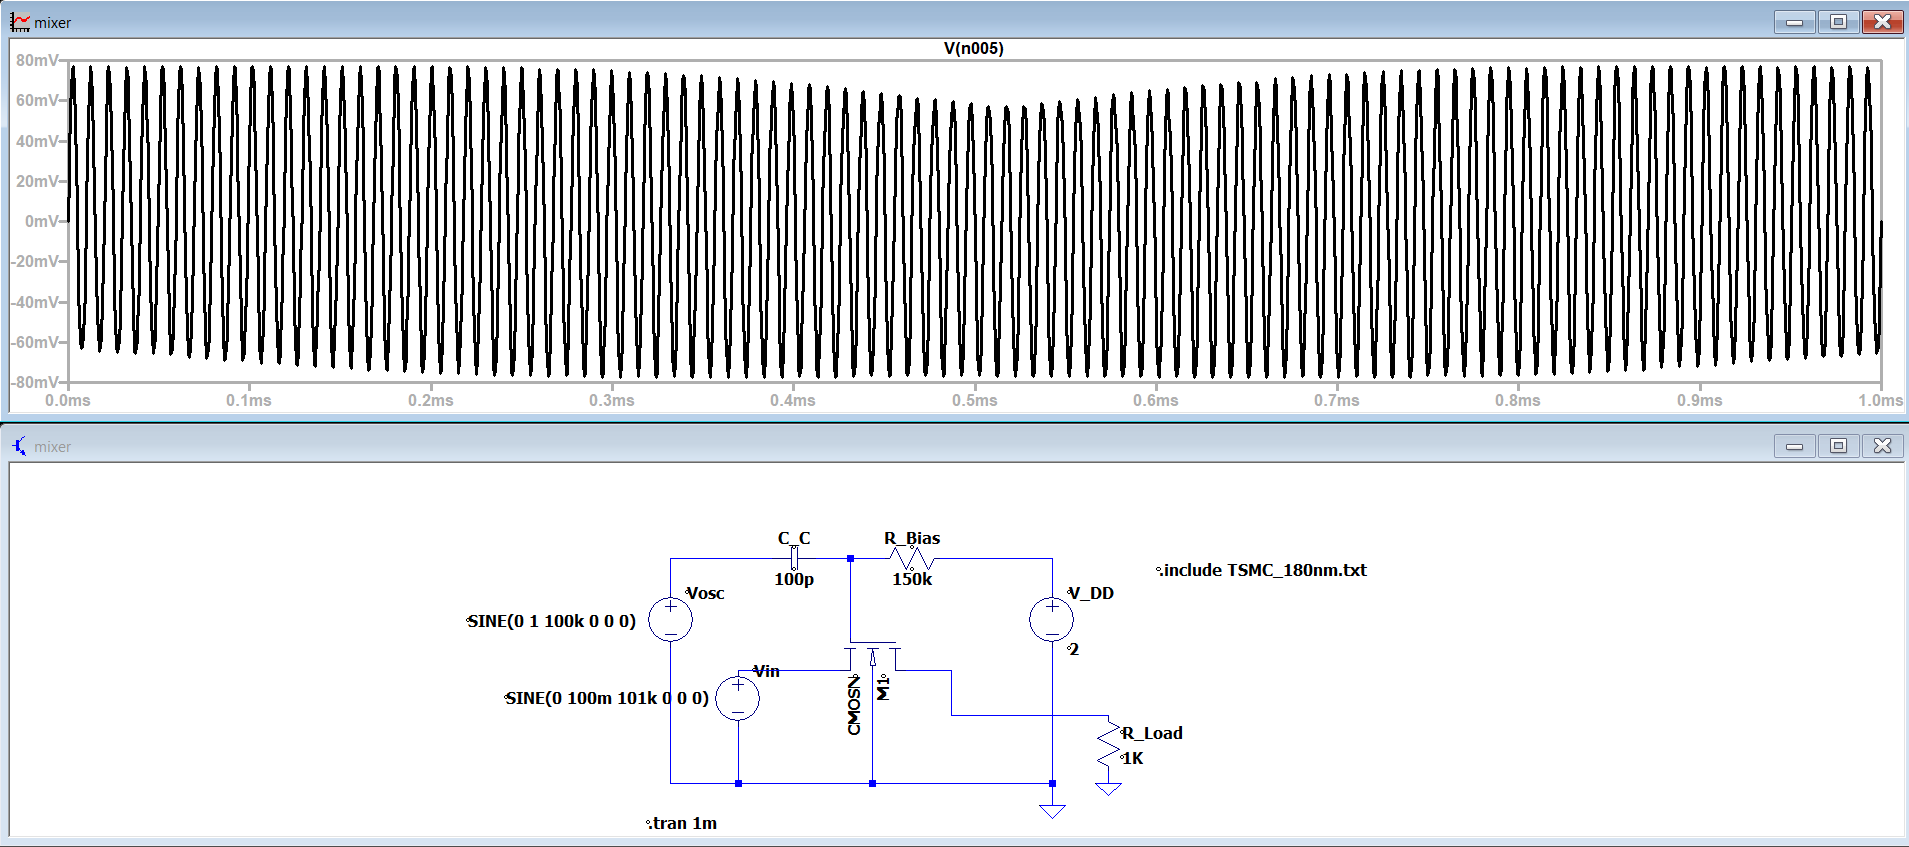
\includegraphics[width=1\linewidth]{fig/101.png}
    \caption{101kHz Output Signal}
    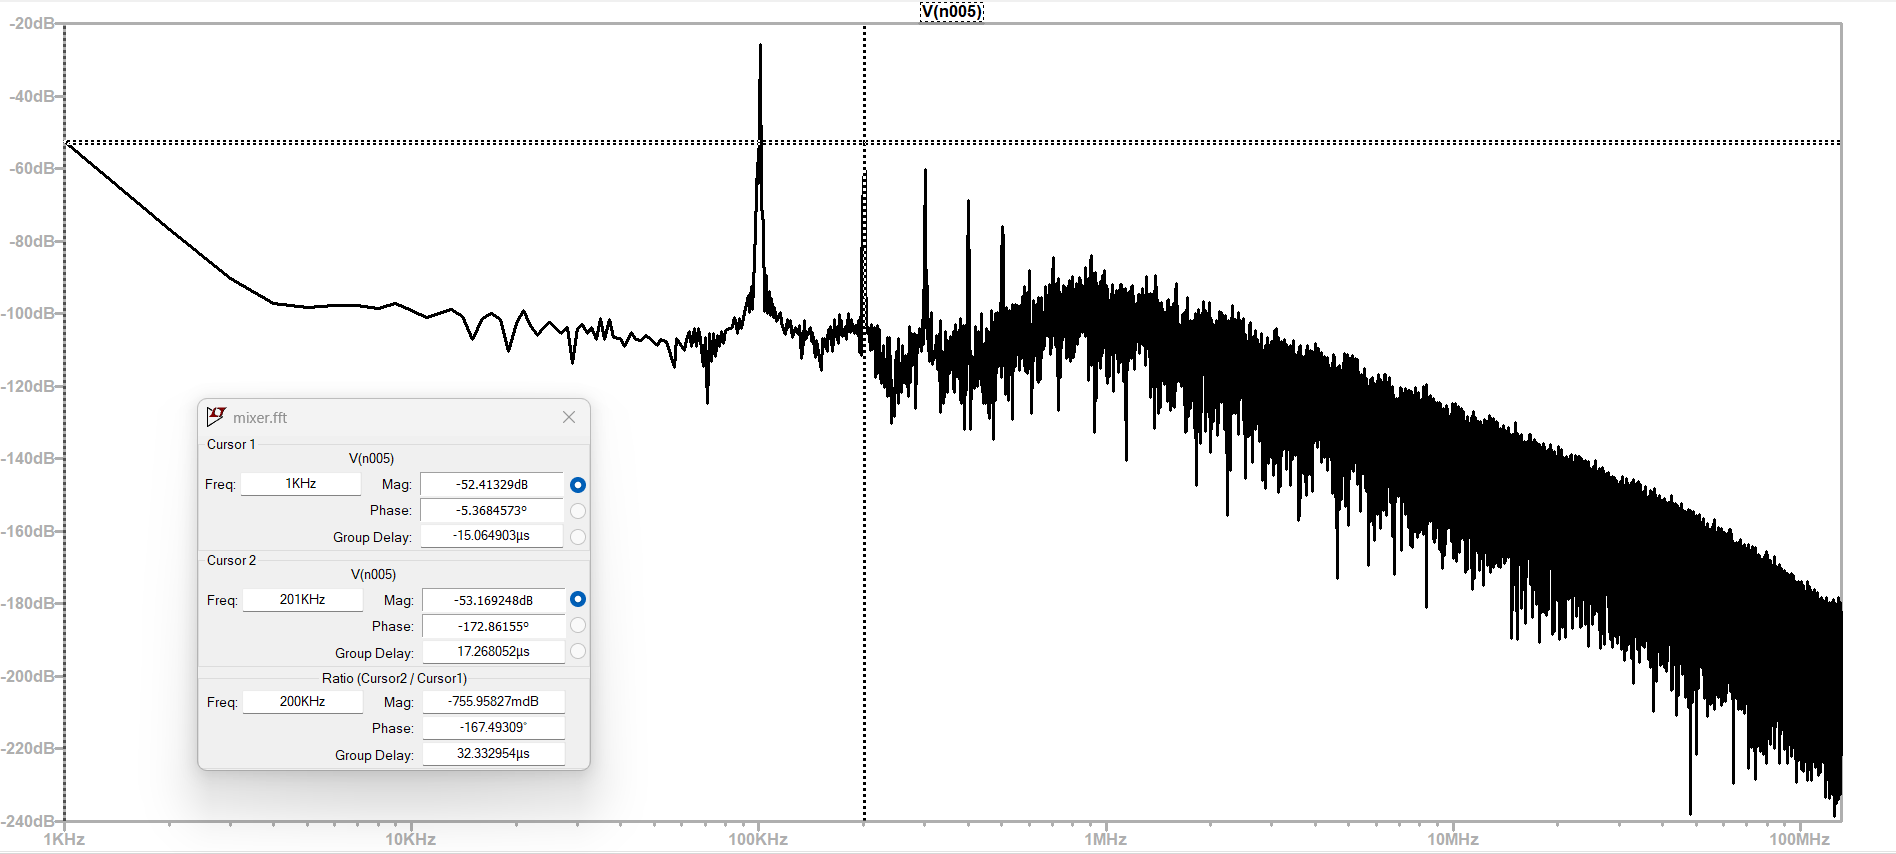
\includegraphics[width=1\linewidth]{fig/101fft.png}
    \caption{101kHz FFT}
\end{figure}
\begin{figure}
    \centering
    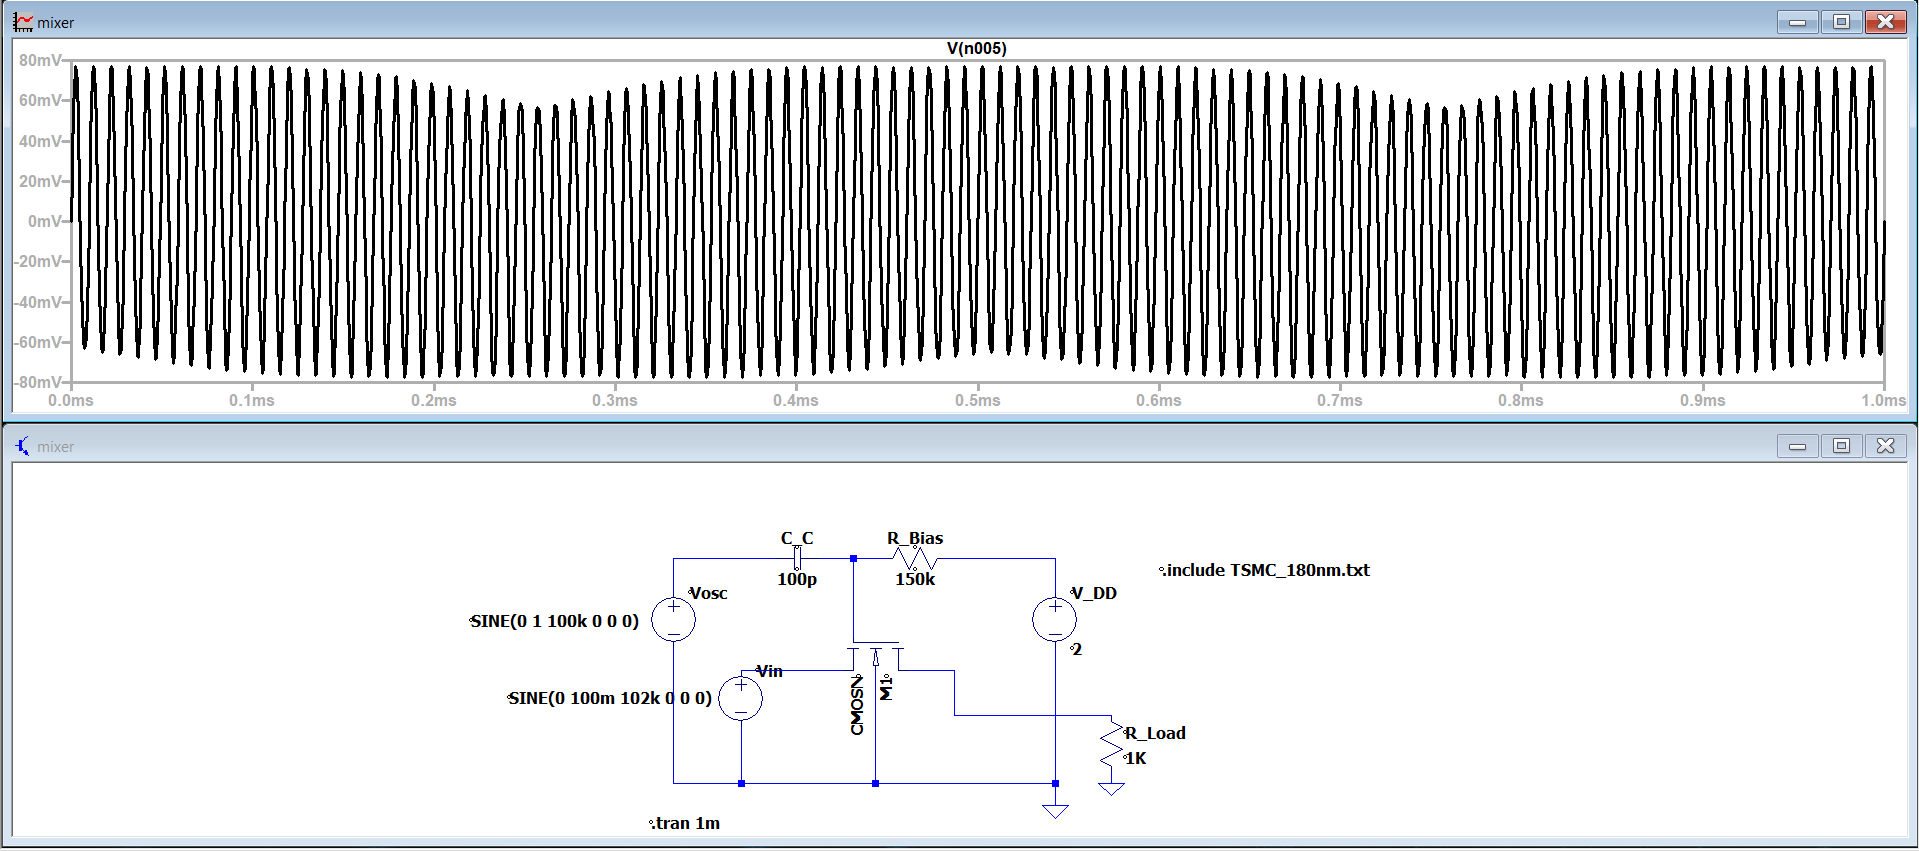
\includegraphics[width=1\linewidth]{102.png}
    \caption{102kHz Output Signal}
    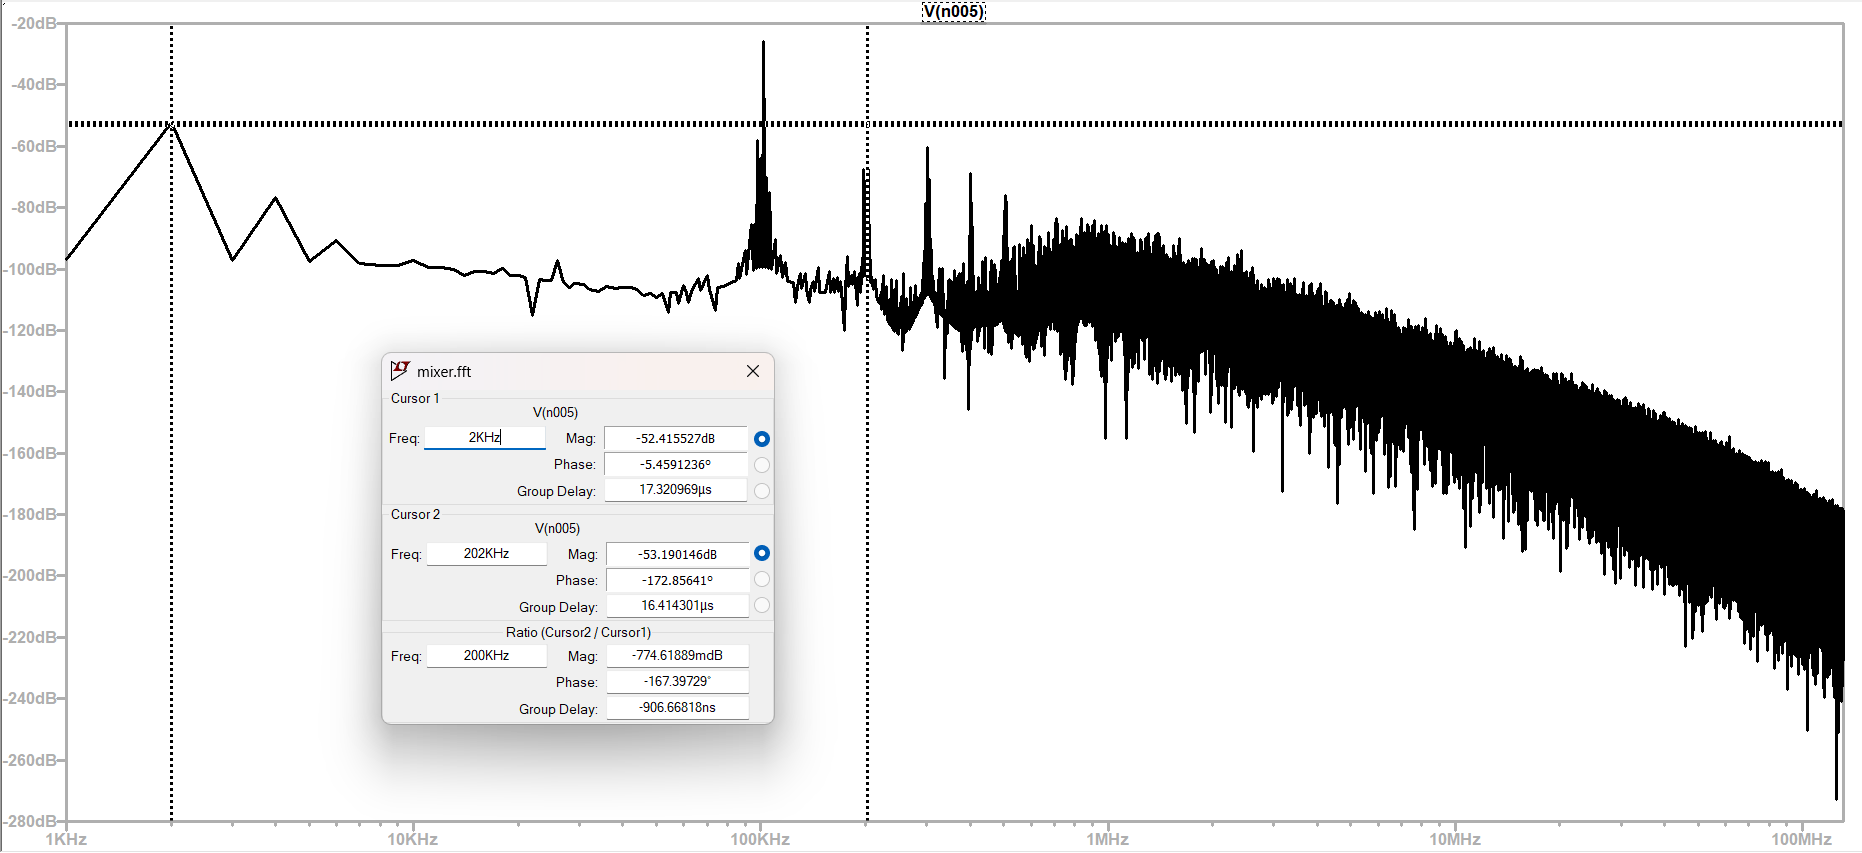
\includegraphics[width=1\linewidth]{fig/102fft.png}
    \caption{102kHz FFT}
\end{figure}
Our observations from these simulations reveal:

\begin{itemize}
    \item For $f_{in} < f_{osc}$ (when $\Delta f$ is negative): The IF signal has reversed phase compared to input.
    \item For $f_{in} > f_{osc}$ (when $\Delta f$ is positive): The IF signal maintains same phase relationship.
    \item In all cases, the difference frequency $|\Delta f| = |f_{in} - f_{osc}|$ clearly appears in the output.
    \item The FFT analysis confirms the presence of all expected frequency components:
        \begin{itemize}
            \item Difference frequency ($|\Delta f|$)
            \item Sum frequency ($f_{in} + f_{osc}$ or $2f_{osc} + \Delta f$)
            \item Input frequency leakage ($f_{in}$ or $f_{osc} + \Delta f$)
            \item LO leakage ($f_{osc}$)
        \end{itemize}
\end{itemize}
\subsection{Analysis of Phase Relationships and Image Frequency Problem}

An important observation from our mixer simulations with different input frequencies is the behavior when using input signals equidistant from the LO frequency. As shown in Fig.~\ref{fig:nmos_mixer}, we tested the mixer with both $f_{in} = 105$ kHz ($\Delta f = +5$ kHz) and $f_{in} = 95$ kHz ($\Delta f = -5$ kHz). Despite having different input frequencies, both produced remarkably similar output waveforms.

\begin{figure}[H]
    \centering
    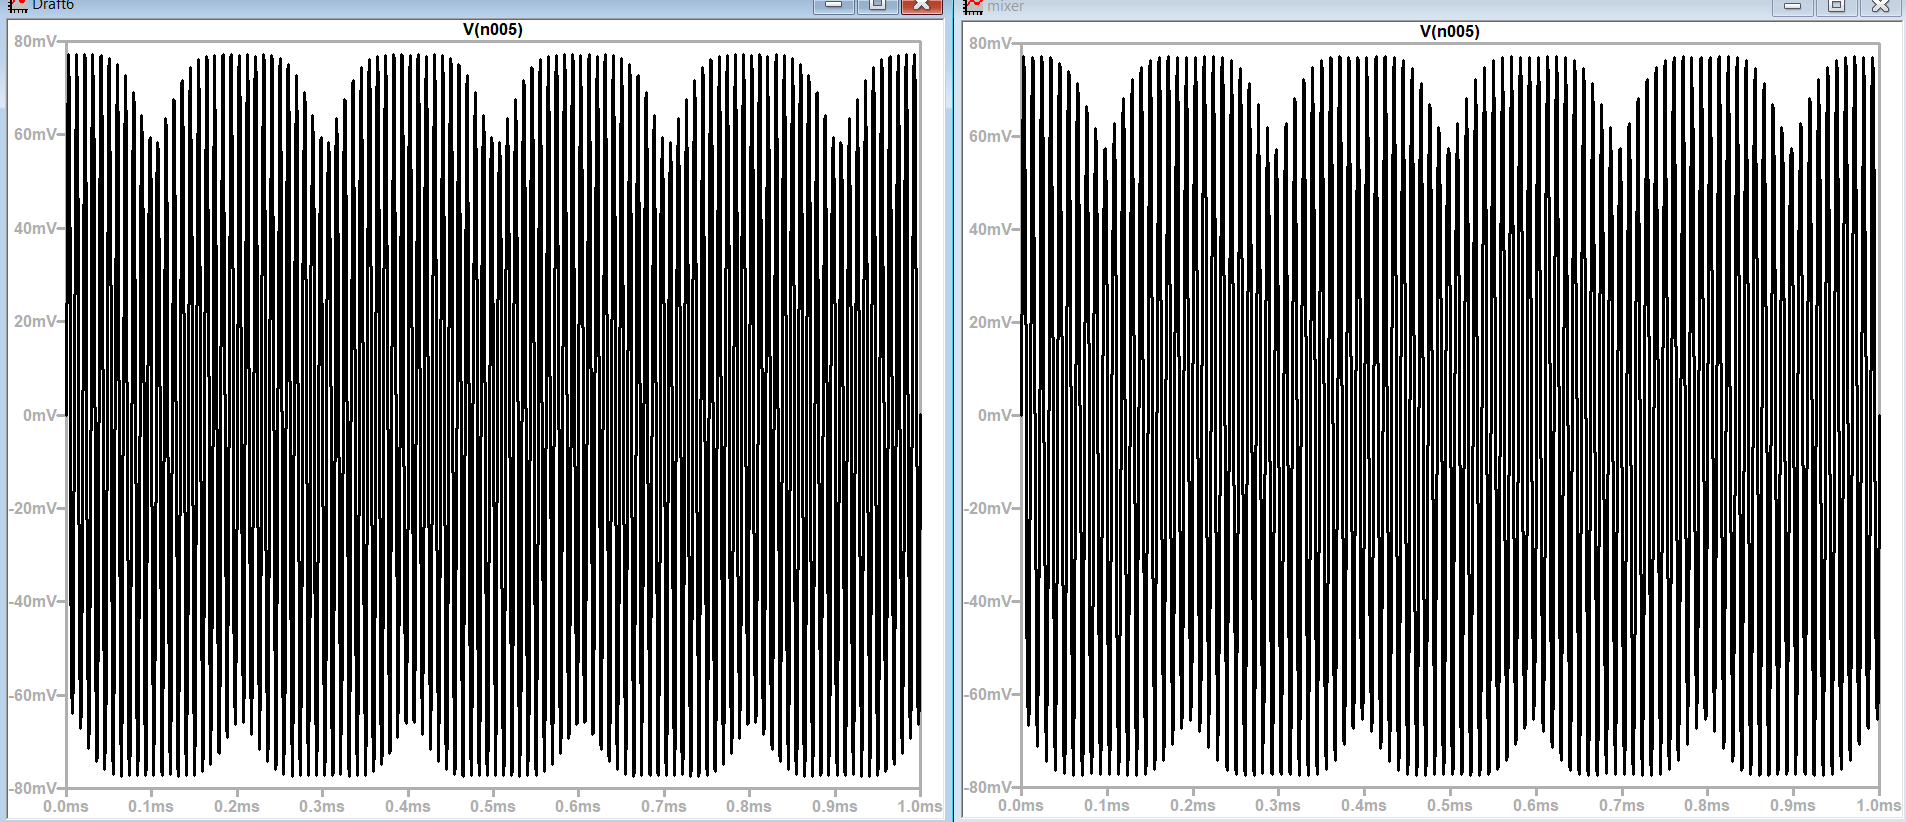
\includegraphics[width=1\linewidth]{fig/compare.png}
    \caption{Comparison of Mixer Outputs for $f_{in} = 105$ kHz and $f_{in} = 95$ kHz}
    \label{fig:image_frequency}
\end{figure}

This similarity occurs because:

\begin{itemize}
    \item Both produce the same absolute intermediate frequency: $|f_{in} - f_{osc}| = 5$ kHz in both cases
    \item Both display identical beat patterns with an envelope frequency of 5 kHz
    \item Both have similar amplitude ranges (approximately $-80$ mV to $+80$ mV)
\end{itemize}

The key difference between these two cases is theoretical rather than visual. When $f_{in} > f_{osc}$ (105 kHz case), the IF signal maintains the same phase relationship as the input, while when $f_{in} < f_{osc}$ (95 kHz case), the IF signal should exhibit a reversed phase.

Mathematically, this phase inversion occurs because when $\Delta f$ is negative, the term $\cos((\omega_{in} - \omega_{osc})t)$ becomes $\cos((\omega_{osc} - \omega_{in})t) = \cos(-(\omega_{in} - \omega_{osc})t) = \cos((\omega_{in} - \omega_{osc})t + \pi)$, introducing a 180° phase shift.

This similarity demonstrates the classic "image frequency" problem in single mixer systems, where two different input frequencies ($f_{osc} \pm \Delta f$) produce nearly identical outputs. This ambiguity between positive and negative frequency offsets highlights the importance of quadrature down-conversion in modern wireless receivers, where the phase relationships between I and Q channels enable discrimination between signals above and below the LO frequency.

These simulation results confirm that our NMOS mixer successfully performs the frequency translation function required for the quadrature down converter, with the output containing the desired intermediate frequency components that can be further processed by the subsequent low-pass filter stage.
